\documentclass{article}
\usepackage[utf8]{inputenc}
\usepackage[a4paper,left=3.5cm,right=3.5cm,top=2cm,bottom=2cm]{geometry}
\usepackage{crop,graphicx,amsmath,array,color,amssymb,fancyhdr,lineno}
\usepackage{flushend,stfloats,amsthm,chngpage,times,,lipsum,lastpage} 
\usepackage{calc,listings,color,wrapfig,tabularx,longtable,enumitem}
\usepackage{multirow}
\usepackage{caption}
\usepackage{subcaption}
\usepackage{xcolor}
\usepackage{tcolorbox}
\definecolor{shadecolor}{rgb}{0.86,0.86,0.86}
\usepackage{float}
\usepackage{lineno}
\usepackage{csquotes}
\usepackage[italian]{babel}
\usepackage[hidelinks]{hyperref}

\pagestyle{fancy}
\fancypagestyle{plain}{%
  \renewcommand{\headrulewidth}{0pt}%
  \fancyhf{}%
}

\title{Confronto tra Algoritmi di String Matching}
\author{Eros Pinzani}

\begin{document}

\begin{titlepage}
    \centering
    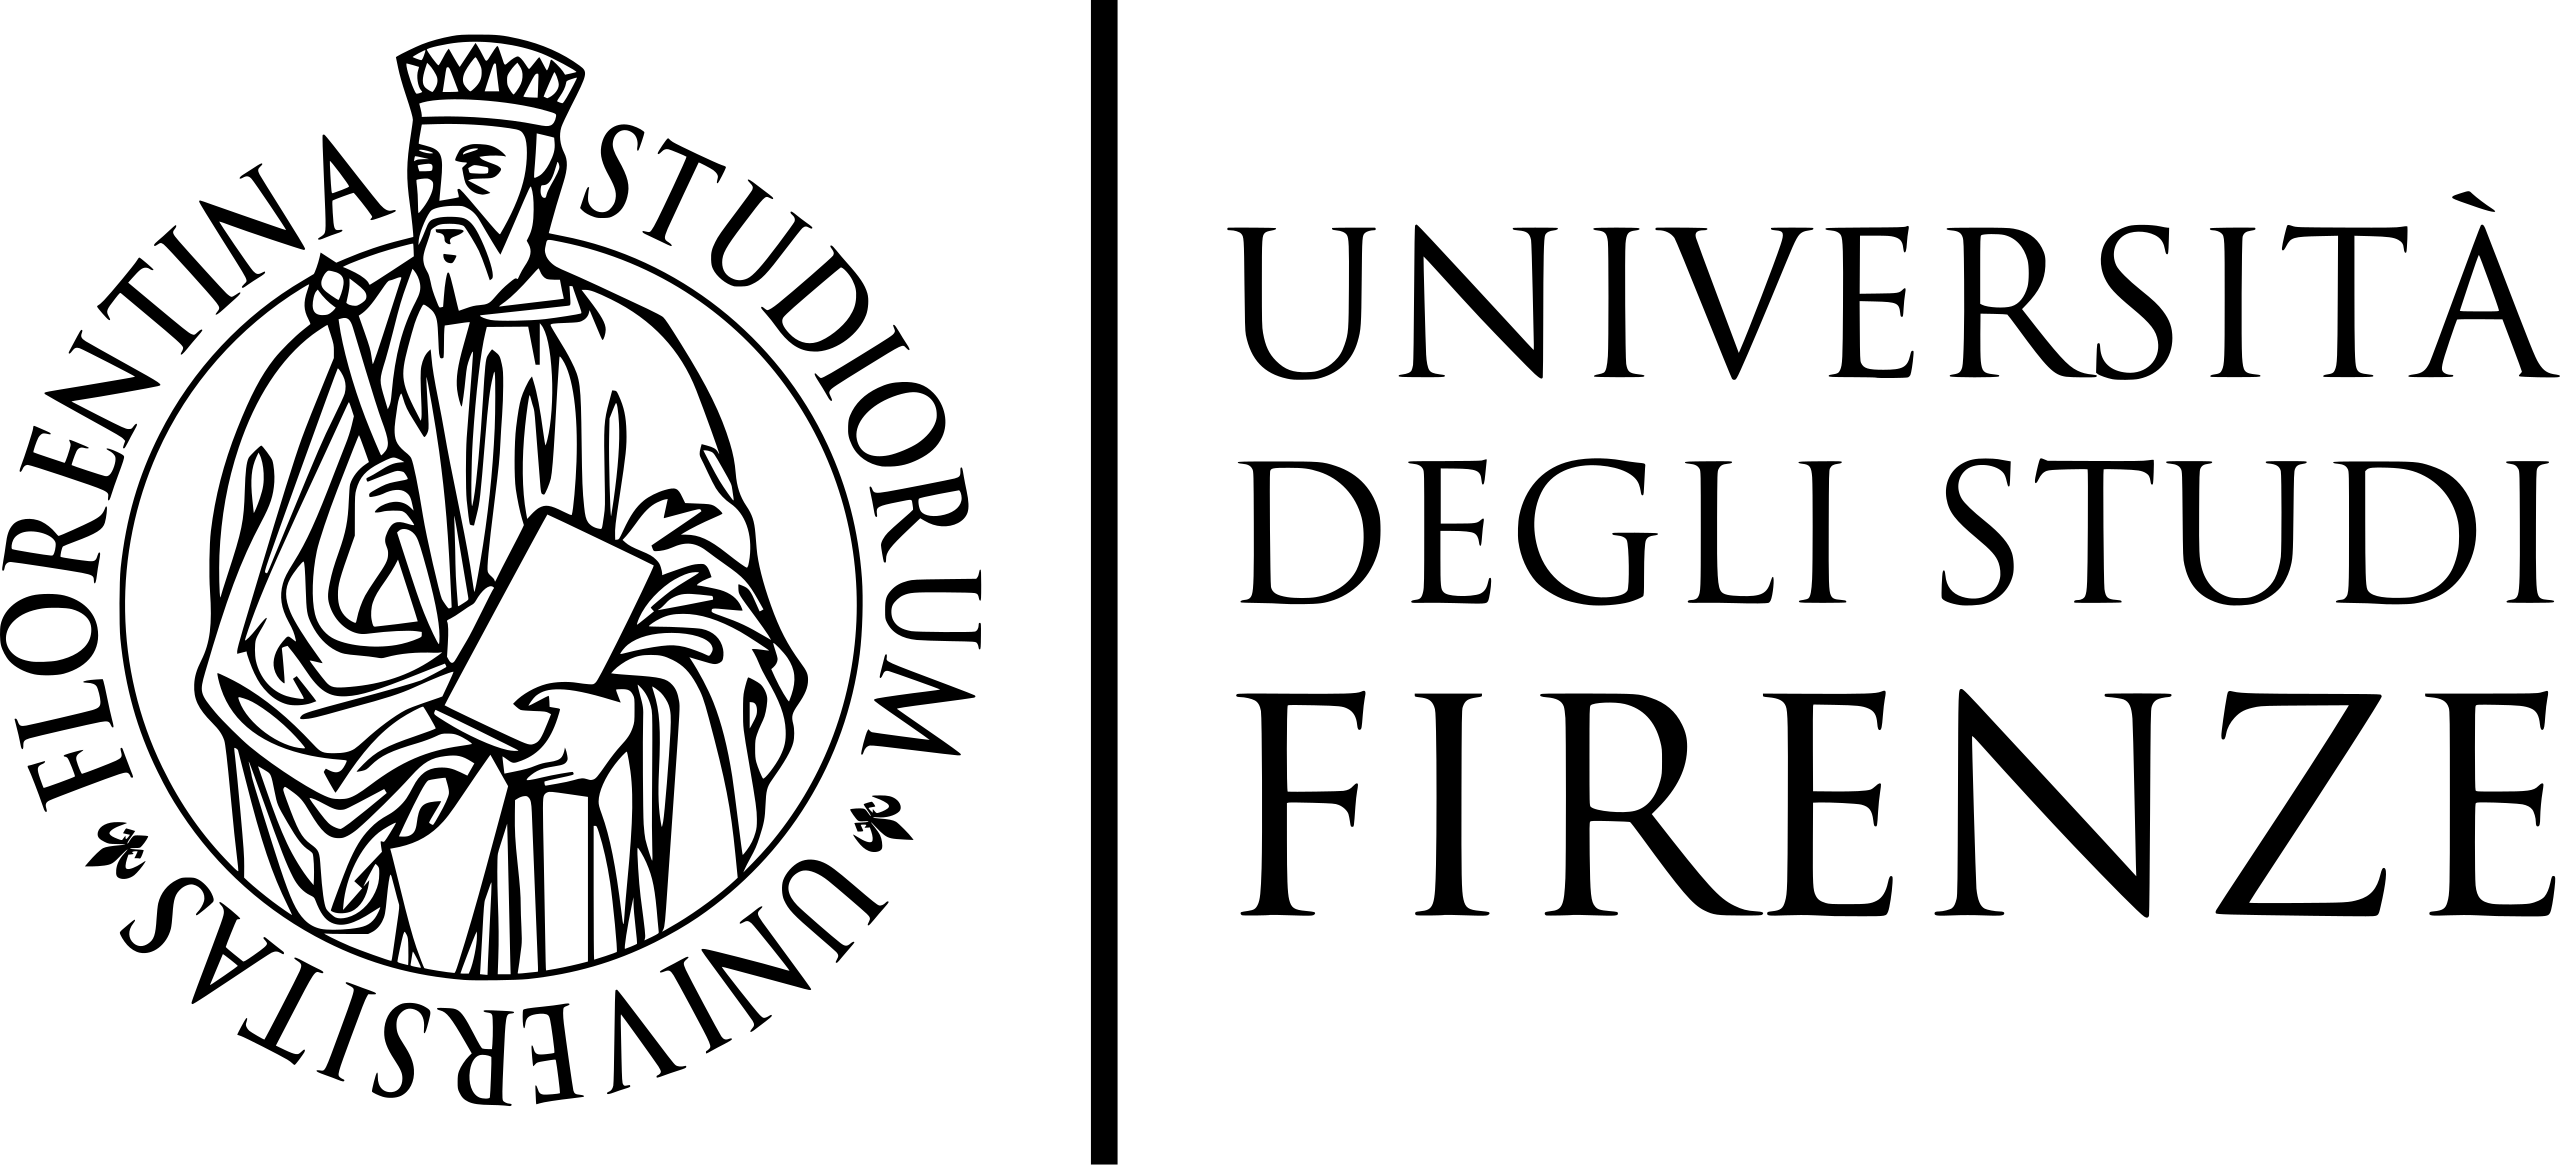
\includegraphics[width=0.90\textwidth]{img/Logo_universita_firenze.svg.png}\par\vspace{1cm}
    {\scshape\LARGE Università degli Studi di Firenze \par}
    \vspace{0.25cm}
    {\scshape\Large Dipartimento di Ingegneria dell'Informazione\par}
    \vspace{0.5cm}
    \rule{\linewidth}{0.4pt}
    \begin{center}
        {\Huge{\bfseries \textbf{Confronto tra Algoritmi di String Matching}\par}}
    \end{center}
    \rule{\linewidth}{0.4pt}
    \vspace{1cm}

    \begin{minipage}[t]{0.4\textwidth}
        \begin{flushleft} \large
            \emph{Autore:}\par
            Eros Pinzani\par
        \end{flushleft}

        \begin{flushleft} \large
            \emph{N° Matricola:}\par
            7030989\par
        \end{flushleft}
    \end{minipage}
    \hfill
    \begin{minipage}[t]{0.4\textwidth}
        \begin{flushleft} \large\raggedleft
            \emph{Corso:}\par
            Algoritmi e Strutture Dati
        \end{flushleft}

        \begin{flushleft} \large\raggedleft
            \emph{Docente corso:}\par
            Simone Marinai\par
        \end{flushleft}
    \end{minipage}

\end{titlepage}

\newpage
\renewcommand{\contentsname}{Indice}
\tableofcontents
\pagenumbering{arabic}
\newpage
\section{Introduzione generale}
\subsection{Breve descrizione dello svolgimento degli esercizi}
Per ogni esercizio suddividiamo la sua descrizione in 4 parti fondamentali:

\begin{itemize}
    \item \textbf{Spiegazione teorica del problema} : qui è dove si descrive il problema che andremo ad affrontare in modo teorico partendo dagli assunti del libro di Algoritmi e Strutture Dati e da altre fonti.
    \item \textbf{Documentazione del codice} : in questa parte spieghiamo come il codice dell'esercizio viene implementato.
    \item \textbf{Descrizione degli esperimenti condotti} : partendo dal codice ed effettuando misurazioni varie cerchiamo di verificare le ipotesi teoriche.
    \item \textbf{Analisi dei risultati sperimentali} : dopo aver svolto i vari esperimenti riflettiamo sui vari risultati ed esponiamo una tesi.
\end{itemize}

\subsection{Specifiche della piattaforma di test}
La piattaforma di test sarà la stessa per ogni esercizio che vedremo. Partiamo dall'hardware del computer fondamentale da conoscere per questo esercizio:

\begin{itemize}
    \item \textbf{CPU} : AMD Ryzen™ 5 PRO 7540U (da 3,2 GHz fino a 4,9 GHz)
    \item \textbf{RAM} : 16 GB LPDDR5X-6.400MT/s
    \item \textbf{SSD} : 512 GB M.2 2280 PCIe Gen4 TLC Opal
\end{itemize}

Il linguaggio di programmazione utilizzato sarà Python e la piattaforma in cui il codice è stato scritto e 'girato' è l'IDE \textbf{Visual Studio Code}. La stesura di questo testo è avvenuta tramite l'utilizzo di \textbf{Visual Studio Code} e opportune estensioni.

\part{Algoritmo ``ingenuo'' vs Algoritmo KMP}

\begin{tcolorbox}[colback=lightgray!20,
                  colframe=black,
                  arc=3mm, auto outer arc,]
                  
    \textbf{Esercizio A}
    \begin{itemize}
    
    \item Vogliamo confrontare gli algoritmi ``ingenuo'' e KMP per effettuare string matching
    
    \item Per fare questo dovremo:
    
        \begin{itemize}
          
            \item Scrivere i programmi Python che:
          
            \begin{itemize}
            
                \item implementino quanto richiesto
                
                \item eseguono un insieme di test che ci permettano di comprendere vantaggi e svantaggi delle diverse implementazioni
                
            \end{itemize}
                
            \item Svolgere ed analizzare opportuni esperimenti
            
            \item Scrivere una relazione che descriva quanto fatto
            
        \end{itemize}
        
    \end{itemize}
\end{tcolorbox}

\end{document}